\documentclass[10pt]{beamer}

\usetheme[progressbar=frametitle]{metropolis}

\usepackage{booktabs}
\usepackage[scale=2]{ccicons}

\usepackage{pgfplots}
\usepgfplotslibrary{dateplot}

\usepackage{xspace}
\newcommand{\themename}{\textbf{\textsc{metropolis}}\xspace}

\usepackage{tikz}
\usetikzlibrary[topaths]

\usepackage{wasysym}

\title{Popularity, Mixed Matchings, and Self-duality}
\subtitle{Chien-Chung Huang and Telikepalli Kavitha}
\date{\today}
\author{Justin Toth}
\institute{University of Waterloo}
%\titlegraphic{\hfill\includegraphics[height=1.5cm]{logo}}

%Macros
\newcommand{\A}{\mathbb{A}}
\newcommand{\D}{\mathbb{D}} \newcommand{\F}{\mathbb{F}}
\newcommand{\N}{\mathbb{N}} \newcommand{\R}{\mathbb{R}}
 \newcommand{\Z}{\mathbb{Z}}
\newcommand{\Q}{\mathbb{Q}}
 
 
\newcommand{\cA}{\mathcal{A}} \newcommand{\cB}{\mathcal{B}}
\newcommand{\cC}{\mathcal{C}} \newcommand{\cD}{\mathcal{D}}
\newcommand{\cE}{\mathcal{E}} \newcommand{\cF}{\mathcal{F}}
\newcommand{\cG}{\mathcal{G}} \newcommand{\cH}{\mathcal{H}}
\newcommand{\cI}{\mathcal{I}} \newcommand{\cJ}{\mathcal{J}}
\newcommand{\cK}{\mathcal{K}} \newcommand{\cL}{\mathcal{L}}
\newcommand{\cM}{\mathcal{M}} \newcommand{\cN}{\mathcal{N}}
\newcommand{\cO}{\mathcal{O}} \newcommand{\cP}{\mathcal{P}}
\newcommand{\cQ}{\mathcal{Q}} \newcommand{\cR}{\mathcal{R}}
\newcommand{\cS}{\mathcal{S}} \newcommand{\cT}{\mathcal{T}}
\newcommand{\cU}{\mathcal{U}} \newcommand{\cV}{\mathcal{V}}
\newcommand{\cW}{\mathcal{W}} \newcommand{\cX}{\mathcal{X}}
\newcommand{\cY}{\mathcal{Y}} \newcommand{\cZ}{\mathcal{Z}}

\newcommand\numberthis{\addtocounter{equation}{1}\tag{\theequation}}



\newcommand{\size}[1]{\ensuremath{\left|#1\right|}}
\newcommand{\ceil}[1]{\ensuremath{\left\lceil#1\right\rceil}}
\newcommand{\floor}[1]{\ensuremath{\left\lfloor#1\right\rfloor}}

%END MACROS

\begin{document}
\setbeamercolor{background canvas}{bg=white}
\maketitle

\section{Introduction}

\begin{frame}
\frametitle{Voting}
Consider a graph $\alert{G = (V,E)}$, and a matching $\alert{M}$ on $\alert{G}$.

We define the vote of $\alert{u}$ for $\alert{v}$ versus $\alert{v'}$ as
$$vote_u(v,v') = \begin{cases}
1, &\text{if $u$ prefers $v$ to $v'$} \\
-1, &\text{if $u$ prefers $v'$ to $v$} \\
0, &\text{otherwise}
\end{cases}
$$
We can aggregate the margin of victory in an election between two matchings $\alert{M}$ and $\alert{M'}$ by
$$\Delta(M,M') := \sum_{u \in V(G)} vote_u(M(u), M'(u)) $$
where $\alert{M(u)}$ denotes the partner of $\alert{u}$ in $\alert{M}$.
\end{frame}

\begin{frame}
\frametitle{Popular Matchings}
We call $\text{\alert{M}}$ a $\text{\alert{popular}}$ matching if it never loses elections:
$$\forall \text{matchings } M', \quad \Delta(M,M') \geq 0.$$


The max utility popular matching problem $\text{\alert{(MaxPM)}}$ asks to find a $\text{\alert{popular}}$ matching $\alert{M}$ on $\alert{G}$ which maximizes
$$\sum_{e\in M} w(e)$$
for some weights $\alert{ w: E(G) \rightarrow \Q_+}$.
\end{frame}

\begin{frame}
\frametitle{Fractional Matchings}
We can extend this to the $\text{\alert{fractional matching}}$ case:
$$FM_{G} = \{x \in \R^m_+ : x(\delta(u)) \leq 1, \forall u \in V(G)\}.$$
We extend the voting function by defining for all $\alert{x \in FM_G}$, for all $\alert{u,v' \in V(G)}$:
$$vote_u(x,v) = \sum_{uv'\in \delta(u)} x_{uv'} vote_u(v',v) \text{ and } vote_u(v,x) = -vote_u(x,v).$$ 
We extend the vote aggregation defining for all $\alert{x, y \in FM_{G}}$:
$$\Delta(x,y) = \sum_{u \in V(G)} \sum_{uv \in \delta(u)} x_{uv}vote_u(v,y).$$
The polytope of all $\text{\alert{fractional popular matchings}}$ is 
$$P_G := \{x \in FM_{G}: \Delta(x,y) \geq 0, \forall y \in FM_G\}.$$
\end{frame}

\begin{frame}
\frametitle{Mixed Popular Matching Example}
In $\text{\alert{bipartite}}$ graphs, each $\alert{x \in FM_G}$ is a convex combination of matchings. But each $\alert{x\in P_G}$ need not be a convex combination of $\text{\alert{popular}}$ matchings.
\begin{columns}[T] % align columns
\begin{column}{.48\textwidth}
\begin{figure}
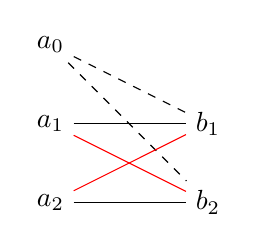
\begin{tikzpicture} 
\node[] (a0) at (0,5) {$a_0$};
    \node[] (a1) at (0,4) {$a_1$};
    \node[] (a2) at (0,3) {$a_2$};
    
    \node[] (b1) at (2,4) {$b_1$};
    \node[] (b2) at (2,3) {$b_2$};
    
    \path[dashed] (a0) edge (b1);
    \path[dashed] (a0) edge (b2);
    \path[-] (a1) edge (b1);
    \path[-] (a2) edge (b2);
    \path[-,red] (a1) edge (b2);
    \path[-,red] (a2) edge (b1);
\end{tikzpicture}
\end{figure}
\end{column}%
\hfill%
\begin{column}{.48\textwidth}
$$ $$
Say each $\alert{a_i}$ has preferences $\alert{b_1 > b_2}$, and each $\alert{b_i}$ has preferences $\alert{a_1 > a_2 > a_0}$.
\end{column}%
\end{columns}
Solid black edges $\alert{S}$ is the only $\text{\alert{popular}}$ matching. If we let $\alert{M}$ be the solid red edges then $$\Pi= \{(S,\frac{1}{2}), (M,\frac{1}{2})\}$$ is a $\text{\alert{fractional popular matching}}$.
\end{frame}

\begin{frame}
\frametitle{Extended Formulation}
Fix a popular fractional matching $\alert{y}$. Then $\alert{\Delta(x,y)}$ is a linear function in $\alert{x}$. Since $\alert{y}$ is popular $\alert{\Delta(x,y) \leq 0}$ with equality when $\alert{x}$ is popular.
\begin{columns}[T]
\begin{column}{.48\textwidth}
\begin{align*}
\max &\Delta(x,y) \\
\text{s.t.} \sum_{e \in \delta(u)} x_e &= 1 &\forall u \in V(G) \\
x_e &\geq 0 &\forall e \in E
\end{align*}
\end{column}
\begin{column}{.48\textwidth}
\begin{align*}
\min &\sum_{u \in V(G)} \alpha_u  \\
\text{s.t.} \alpha_a + \alpha_b &\geq vote_a(b,y) \\&+ vote_b(a,y) &\forall ab \in E(G) \\
\alpha_u &\geq vote_u(\ell(u), y) &\forall u \in V(G).
\end{align*}
\end{column}
\end{columns}
Where $\alert{\ell(u)}$ is an appended last choice vertex for each $\alert{u}$.

We call $\alert{\alpha}$ such that $\alert{\sum_{u} \alpha_u = 0}$ a witness to the popularity of $\alert{y}$.
\end{frame}

\begin{frame}
\frametitle{Extended Formulation}
From the primal-dual pair we obtain the extended formulation $\alert{(LP)}$:
\begin{align*}
\min &\sum_{u \in V(G)} \alpha_u \\
\text{s.t.} \alpha_a + \alpha_b &\geq vote_a(b,x) + vote_b(a,x) &\forall ab \in E(G) \\
\alpha_u &\geq vote_u(\ell(u),x) &\forall u \in V(G) \\
\sum_{e \in \delta(u)} x_e &=1 &\forall u \in V(G) \\
x_e &\geq 0 &\forall e \in E.
\end{align*}
Optimal value is $0$. The optimal solutions are $\text{\alert{popular matchings}}$ and their $\text{\alert{witnesses}}$ (see Popular Mixed Matchings by Kavitha et al. for details).
\end{frame}

\begin{frame}
\frametitle{Extended Formulation}
Let $\alert{P'_G}$ be the optimal solutions to $\alert{(LP)}$. Then $\alert{P'_G}$ is described by the set of $\alert{(x,\alpha)}$ such that:
\begin{align*}
\sum_{u \in V(G)} \alpha_u &= 0 \\
 \alpha_a + \alpha_b &\geq vote_a(b,x) + vote_b(a,x) &\forall ab \in E(G) \\
\alpha_u &\geq vote_u(\ell(u),x) &\forall u \in V(G) \\
\sum_{e \in \delta(u)} x_e &=1 &\forall u \in V(G) \\
x_e &\geq 0 &\forall e \in E.
\end{align*}
\end{frame}

\begin{frame}
\frametitle{Self-Duality}
It is straightforward to see that $\alert{(LP)}$ is self-dual (exercise). By $\text{\alert{complementary slackness}}$: the covering constraint for $\alert{ab}$ is tight when $\alert{x_{ab} > 0}$ for any popular fractional matching $\alert{x}$.

$\textbf{Lemma 1}$: For any $\alert{(x,\alpha) \in P'_G}$, if $\alert{x_{ab} > 0}$ then:
$$\alpha_a + \alpha_b = vote_a(b,x) + vote_b(a,x).$$ 
\end{frame}
\section{Integrality of $P_G$ in a special case}
\begin{frame}
\frametitle{Objective}
$\textbf{Theorem 1:}$ If $\alert{G =(A\cup B, E)}$ is $\text{\alert{bipartite}}$ and admits a $\text{\alert{perfect stable matching}}$ then $\alert{P_G}$ is integral.

From prior talks: $\text{\alert{stable matchings}}$ are $\text{\alert{minimum size popular matchings}}$.

Hypothesis says each $\text{\alert{popular matching}}$ is perfect and, in fractional setting, for each $\alert{u\in A \cup B}$, $\alert{x_{u\ell(u)} = 0}$.

To prove $\textbf{Theorem 1}$ we will write $\alert{(x,\alpha^x) \in P_G'}$ as a convex combination of $\text{\alert{popular matchings}}$.
\end{frame}

\begin{frame}
\frametitle{Bounding $\alpha^x$}
$\textbf{Lemma 2:}$ $\alert{\alpha^x \in [-1,1]}$.

$\textbf{Proof:}$ First
$$\alpha^x_u \geq vote_u(\ell(u), x) = -1 \text{(since }x_{u,\ell(u)} = 0\text{).}$$
Now let $\alert{v}$ be the least preferred neighbour of $\alert{u}$ such that $\alert{x_{uv} >0}$. Then
$$vote_u(v,x) = -vote_u(x,v) = -(1-x_{uv}).$$
Also
$$vote_v(u,x) = \sum_{u':u' <_v u} x_{u'v} - \sum_{u':u' >_v u} x_{u'v} = 1-x_{uv}.$$
So by $\textbf{Lemma 1}$
$$\alpha_u + \alpha_v = vote_u(v,x) + vote_v(u,x) \leq -(1-x_{uv}) + (1-x_{uv}) = 0.$$
Since $\alert{\alpha_v \geq -1}$ this implies $\alert{\alpha_u \leq 1}$.$\blacksquare$
\end{frame}

\begin{frame}
\frametitle{Constructing the Table: $a \in A$}
\centering
$r_a\cdot 1 + (1-r_a)(-1) = \alpha^x_a$ 
\includegraphics[scale=0.25]{Xa}

For each $\alert{ab \in \delta(a)}$ create a cell of length $\alert{x_{ab}}$ (omit $0$-length cells) and arrange cells in increasing order (w.r.t. $\alert{a}$) to form $\alert{X_a}$.
\end{frame}

\begin{frame}
\frametitle{Constructing the Table: $b \in B$}
\centering
$r_b(-1) + (1-r_b)\cdot 1 = \alpha^x_b$
\includegraphics[scale=0.25]{Xb}

For each $\alert{ab \in \delta(b)}$ create a cell of length $\alert{x_{ab}}$ (omit $0$-length cells) and arrange cells in decreasing order (w.r.t. $\alert{b}$) to form $\alert{X_b}$.
\end{frame}

\begin{frame}
\frametitle{Constructing the Table: Finding Matchings}
We form the table $\alert{T}$ whose rows are the arrays $\alert{X'_u}$ for each $\alert{u \in V(G)}$.

For any $\alert{t \in [0,1)}$ form $\alert{M_t\subseteq E}$ as follows:
\begin{enumerate}
\item Draw a vertical line at distance $\alert{t}$ from left end of $\alert{T}$.
\item For each $\alert{u \in V(G)}$ define $\alert{c_u(t)}$ to be the cell in $\alert{X'_u}$ which the line intersects (or touches the left boundary of).
\item Set $\alert{M_t = \{ uv \in E(G) : u \in V(G) \text{ and } v \in c_u(t)\}}$.
\end{enumerate}

We claim that each $\alert{M_t}$ is a $\text{\alert{popular matching}}$.
\end{frame}

\begin{frame}
\frametitle{Brief detour to pick up a Lemma}
$\textbf{Lemma 3}$ For any $\alert{ab \in E(G)}$,
$$ x_{ab} + \sum_{b' <_a b} x_{ab'} + \sum_{a' <_b a} x_{a'b} \leq r_a + (1-r_b).$$
Equality holds if $\alert{x_{ab} > 0}$.

$\textbf{Proof:}$
From the covering constraint for $\alert{P'_G}$:
$$\alpha^x_a + \alpha^x_b \geq \sum_{b' <_a b} x_{ab'} - \sum_{b' >_a b} x_{ab'} + \sum_{a' <_b a} x_{a'b} - \sum_{a' >_b a} x_{a'b}.$$
Substitute $\alert{\sum_{b' >_a b} x_{ab'} = 1- x_{ab} - \sum_{b'<_a b} x_{ab'}}$, and similar for $\alert{\sum_{a' >_b a}x_{a'b}}$. Substitute $\alert{\alpha^x_a = 2r_a -1}$ and $\alert{\alpha^x_b = 1-2r_b}$.

The result follows. $\textbf{Lemma 1}$ yields equality when $\alert{x_{ab}} > 0$.$\blacksquare$
\end{frame}

\begin{frame}
\frametitle{$M_t$ is a matching}
$\textbf{Strategy:}$
\begin{enumerate}
\item Consider some edge $\alert{ab}$ such that $\alert{x_{ab} > 0}$.
\item Want to show that $\alert{b \in c_t(a) \iff a \in c_t(b)}$ for any $\alert{t \in [0,1)}$.
\item Will show that the $\alert{ab}$ cell in rows $\alert{X'_a}$ and $\alert{X'_b}$ is perfectly aligned in table $\alert{T}$.
\end{enumerate}

$\textbf{Recall:}$
\begin{itemize}
\item In $\alert{X'_a}$: $\alert{a}$'s increasing order start from $\textit{left}$ of blue subarray (wraps around).
\item In $\alert{X'_b}$: $\alert{b}$'s increasing order starts from $\textit{right}$ of blue subarray (wraps around).
\end{itemize}
\end{frame}

\begin{frame}
\frametitle{$M_t$ is a matching}
$\textbf{Case 1: }$ $\alert{\sum_{b' <_a b} x_{ab'} \geq r_a}$
\begin{columns}[T] % align columns
\begin{column}{.48\textwidth}
\includegraphics[scale=0.23]{geqRa}
\end{column}
\begin{column}{.48\textwidth}
$$ $$
$\quad\quad d:= \sum_{b' <_a b} x_{ab'} -r_a$

$\quad\quad d':=\sum_{a'<_b a} x_{a'b}$

$\quad\quad$By $\textbf{Lemma 3}$:
$$d + x_{ab} + d' = 1-r_b.$$
\end{column}
\end{columns}
The $\textbf{case}$ where $\alert{\sum_{a'<_b a} x_{a'b} \geq (1-r_b)}$ is symmetric.
\end{frame}

\begin{frame}
\frametitle{$M_t$ is a matching}
$\textbf{Case 2: }$ $\alert{\sum_{b' <_a b} x_{ab'} < r_a}$ and $\alert{\sum_{a' <_b a} x_{a'b} < 1 - r_b}$.

In this case, the $\alert{ab}$ cell has been split in $\alert{X'_a}$ and $\alert{X'_b}$.
\begin{columns}[T] % align columns
\begin{column}{.48\textwidth}
\includegraphics[scale=0.23]{lessRa}
\end{column}
\begin{column}{.48\textwidth}
$$ $$
$\quad\quad d_0:= \sum_{b' <_a b} x_{ab'} $

$\quad\quad d_1:=\sum_{a'<_b a} x_{a'b}$

$\quad\quad x^0_{ab} := \text{hatched blue of }X'_a.$

$\quad\quad x^1_{ab} := \text{hatched blue of }X'_b.$

$\quad\quad$By $\textbf{Lemma 3}$:
$$d_0 + x_{ab} + d_1 = r_a + 1-r_b.$$
\end{column}
\end{columns}
\centering
Hence $\alert{x_{ab} + r_a - x^0_{ab}  + (1-r_b) - x^1_{ab} = r_a + (1-r_b)}$, and so $\alert{x_{ab} = x^0_{ab} + x^1_{ab}}$.
\end{frame}
\begin{frame}
\frametitle{$M_t$ is popular}
$\textbf{Strategy:}$
\begin{enumerate}
\item Exhibit a witness vector $\alert{\alpha^t}$ which satisfies $\alert{P'_G}$.
\item For each $\alert{u \in A\cup B}$ if vertical line intersects $\alert{c_t(u)}$ in blue (positive) subarray set $\alert{\alpha^t_u = 1}$
\item Otherwise, in red (negative) subarray, set $\alert{\alpha^t_u = -1}$.
\end{enumerate}
From previous proof, for any $\alert{ab \in M_t}$:

$\quad\alert{c_t(a)}$ is positive if and only if $\alert{c_t(b)}$ is negative.

So then $\alert{\sum_{u \in A\cup B} \alpha^t_u = 0}$. Here we used that $\alert{M_t}$ is perfect. Remains to verify covering constraints.
\end{frame}

\begin{frame}
\frametitle{$M_t$ is popular}
Want to show $\alert{\forall ab \in E(G)}$, $\alert{\alpha^t_a + \alpha^t_b \geq vote_a(b,M_t(a)) + vote_b(a, M_t(b))}.$
We do a case analysis on the ``colours" of $\alert{c_t(a)}$ and $\alert{c_t(b)}$:
\begin{columns}[T] % align columns
\begin{column}{.48\textwidth}
\begin{enumerate}
\item If exactly one of $\alert{c_t(a)}$ or $\alert{c_t(b)}$ is positive then either $\alert{ab \in M_t}$ or at least one of $\alert{a,b}$ is matched to someone better.
\item If both $\alert{c_t(a)}$ and $\alert{c_t(b)}$ are negative then both $\alert{a}$ and $\alert{b}$ get matched to someone better.
\item If both $\alert{c_t(a)}$ and $\alert{c_t(b)}$ are positive their coverage is trivial (RHS $\leq 2$).
\end{enumerate}
\end{column}
\begin{column}{.48\textwidth}
\includegraphics[scale=0.2]{covering}
\end{column}
\end{columns}
\end{frame}

\begin{frame}
\frametitle{Sweeping Procedure}
We write $\alert{x}$ as a convex combination of $\text{\alert{popular matchings}}$:
\begin{enumerate}
\item Initialize $\alert{i=0}$.
\item Sweep a vertical line from left to right across $\alert{T}$. Denote its distance by $\alert{t}$. 
\item Whenever a new cell is encountered fix matching $\alert{M^i = M_t}$ and fix $\alert{t_i = t}$. 
\end{enumerate}
Say we find $\alert{k}$ such matchings. We can then write $\alert{x}$ as:
$$x = t_1\chi(M^0) + (t_2 - t_1)\chi(M^1) + \dots + (1 - t_{k-1}) \chi(M^{k-1}).$$
\end{frame}
\section{Half-Integrality of $P_G$ in a general instance}

\begin{frame}
\frametitle{Constructing Bipartite Instance}
\begin{center}
From a graph $\alert{G}$ we can construct its bipartite graph $\alert{H}$:
\begin{columns}[T]
\begin{column}{.48\textwidth}
\centering
Preferences corresponding to $\textbf{a:} \alert{b} > \alert{c}$ in $\alert{H}$:
$$\textbf{a:} \alert{b'} > \alert{c'} > \alert{a'}$$
$$\textbf{a':} \alert{b}>\alert{c} > \alert{a}.$$
\end{column}
\begin{column}{.48\textwidth}
\includegraphics[scale=0.125]{bipartite}
\end{column}
\end{columns}
\end{center}
$\textbf{Claim:}$ $\alert{H}$ admits a perfect stable matching. 

$\textbf{Proof:}$ Say stable matching $\alert{S}$ exposes $\alert{u}$.

Then $\alert{S' = \{e' : e\in S\} \cup \{e : e' \in S\}}$ is a stable matching that exposes $\alert{u'}$.

Since stable matchings covers the same vertices, $\alert{S}$ does not cover $\alert{u'}$. 

Thus $\alert{uu'}$ blocks $\alert{S}$. $\blacksquare$
\end{frame}

\begin{frame}
\frametitle{$\frac{1}{2}$-integrality of $P_G$}
By $\textbf{Theorem 1}$, $\alert{P_H}$ is integral.

Let $\alert{(x, \alpha) \in P'_G}$. Define $\alert{f: P_G \rightarrow P_H}$ by
$$f(x) = z \text{ where } z_{uv'}=z_{u'v} =x_{uv} \text{ and } z_{uu'} = x_{u\ell(u)}.$$
Verified by witness $\alert{\beta}$ such that $\alert{\beta_u = \beta_{u'} = \alpha_u}$.
Define $\alert{h: P_H \rightarrow P_G}$ by 
$$h(z) = y \text{ where } y_{uv} = (z_{uv'} + z_{u'v})/2 \text{ and } y_{u\ell(u)} = z_{uu'}.$$
Verified by witness $\alert{\alpha_u = (\beta_u + \beta_u')/2}$.
$$x = h(f(x)) = \sum_{i=0}^{k-1} h(\lambda_i \chi(M^i)) = \sum_{i=0}^{k-1} \lambda_i h(\chi(M^i)).$$
Each $\alert{h(\chi(M^i))}$ is $\frac{1}{2}$-integral. $\blacksquare$
\end{frame}
\section{Conclusions}

\begin{frame}
\frametitle{Optimization Problems and Complexity}
A $\text{\alert{max utility popular matching}}$ can be found in poly-time on $\text{\alert{bipartite graphs}}$ which admit a $\text{\alert{perfect stable matching}}$

Also a $\alert{\frac{1}{2}}$$\text{\alert{-integral fractional popular matching}}$ of max utility can be found on any graph.

By reducing from $\text{\alert{Vertex Cover}}$ they show:
\begin{enumerate}
\item $\text{\alert{(MaxPM)}}$ is $NP$-hard, even when preferences are $\text{\alert{strict}}$, $\text{\alert{complete}}$, and $\alert{w: E \rightarrow \{1,2\}}$, and $\alert{G}$ admits a $\text{\alert{stable matching}}$.
\item Under UGC there is no $O(1)$-approximation algorithm for $\text{\alert{(MaxPM)}}$.
\end{enumerate}
\end{frame}

\begin{frame}
\frametitle{Open Questions}

Can we settle the complexity of $\text{\alert{(MaxPM)}}$ on $\text{\alert{bipartite}}$ graphs?

$$ $$

Is there an algorithm for deciding if a general graph admits a $\text{\alert{popular matching}}$ under $\text{\alert{strict}}$ preferences?

$$ $$
Can we say anything better for $\text{\alert{roommates}}$ instances with a $\text{\alert{perfect stable matching}}$?
\end{frame}

\end{document}
